% !TEX root = task-3-21-4.tex
% Editable task bank. Append new BankTask blocks at the end of the document.
\documentclass[12pt,a4paper]{article}
\usepackage{physics-textbook}
\usepackage{graphicx,needspace}
\usetikzlibrary{decorations.pathmorphing}
\newif\ifShowSolutions
\ifdefined\TutorEdition
  \ShowSolutionstrue
\else
  \ShowSolutionsfalse % Change to \ShowSolutionstrue to display solutions.
\fi
\newcounter{banktask}
\newsavebox{\BankTaskBox}
\newcommand{\BankTaskContent}[3]{%
  \noindent\textbf{\thebanktask.}\quad #2\par
  \ifShowSolutions
    \Needspace{50mm}% Keep the solution heading with its opening text or diagram.
    #3\par
    \ifdefined\TutorEdition
      \ifcsname TutorSource#1\endcsname
        \nopagebreak\smallskip{\small\csname TutorSource#1\endcsname\par}%
      \fi
    \fi
  \fi
}
\newcommand{\BankTask}[3]{%
  \refstepcounter{banktask}\par\medskip
  \sbox{\BankTaskBox}{\begin{minipage}{\linewidth}%
    \BankTaskContent{#1}{#2}{#3}\end{minipage}}%
  \ifdim\dimexpr\ht\BankTaskBox+\dp\BankTaskBox\relax>\dimexpr\textheight-20mm\relax
    \Needspace{35mm}\BankTaskContent{#1}{#2}{#3}%
  \else
    \Needspace{\dimexpr\ht\BankTaskBox+\dp\BankTaskBox\relax}%
    \noindent\usebox{\BankTaskBox}\par
  \fi
  \medskip
}
\begin{document}
\BookSubsection{3.21.4}{Гармонический закон колебаний в контуре}


% Source 468FFB: https://ege.fipi.ru/bank/questions.php?search=1&proj=BA1F39653304A5B041B656915DC36B38&qid=468FFB
\BankTask{468FFB}{
\begin{center}
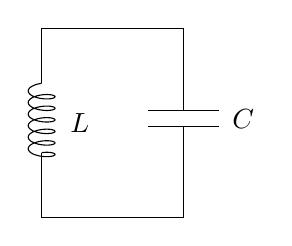
\begin{tikzpicture}[>=stealth,scale=1]
\draw (0,1.7) -- (0,2.4) -- (1.8,2.4) -- (1.8,1.35);
\draw (0,0.7) -- (0,0) -- (1.8,0) -- (1.8,1.15);
\draw (1.35,1.35) -- (2.25,1.35);
\draw (1.35,1.15) -- (2.25,1.15);
\draw (0,0.7) -- (0,0.82);
\draw plot[domain=0:2160,samples=241] ({0.17*sin(\x)},{0.76+0.88*\x/2160+0.06*cos(\x)});
\node[right] at (0.24,1.2) {$L$};
\node[right] at (2.3,1.25) {$C$};
\end{tikzpicture}
\end{center}
В колебательном контуре (см. рисунок) напряжение между обкладками конденсатора меняется по закону $U_C=U_0\cos\omega t$, где $U_0=5\ \text{В}$, $\omega=\pi\cdot10^6\ \text{с}^{-1}$. Определите частоту колебаний силы тока в контуре.

(в $\text{кГц}$).
}{
\smallskip\noindent\textbf{Решение от GPT}\par
Сила тока $I=C\dfrac{dU_C}{dt}=-C U_0\omega\sin\omega t$ имеет ту же циклическую частоту, что и напряжение. Поэтому
\[
\nu=\frac{\omega}{2\pi}=\frac{\pi\cdot10^6}{2\pi}=5\cdot10^5\ \text{Гц}=500\ \text{кГц}.
\]
Ответ: $500$.
}

% Source CFDDFB: https://ege.fipi.ru/bank/questions.php?search=1&proj=BA1F39653304A5B041B656915DC36B38&qid=CFDDFB
\BankTask{CFDDFB}{
Конденсатор, заряженный до разности потенциалов $U$, в первый раз подключили к катушке с индуктивностью $L$, а во второй — к катушке с индуктивностью $4L$. Каково отношение периодов колебаний энергии конденсатора $\dfrac{T_2}{T_1}$ в этих двух случаях? Потерями энергии в контуре пренебречь.
}{
\smallskip\noindent\textbf{Решение от GPT}\par
Энергия конденсатора $W_C=\dfrac{CU^2}{2}\cos^2\omega t$ меняется с периодом $T_W=\dfrac{\pi}{\omega}=\pi\sqrt{LC}$. Следовательно,
\[
\frac{T_2}{T_1}=\sqrt{\frac{4L}{L}}=2.
\]
Ответ: $2$.
}

% Source 0A8805: https://ege.fipi.ru/bank/questions.php?search=1&proj=BA1F39653304A5B041B656915DC36B38&qid=0A8805
\BankTask{0A8805}{
Во сколько раз увеличится частота свободных электромагнитных колебаний в контуре, если площадь пластин конденсатора, входящего в состав контура, уменьшить в \(9\) раз, а индуктивность катушки увеличить в \(4\) раза?
}{
\smallskip\noindent\textbf{Решение от GPT}\par
Ёмкость конденсатора \(C=\varepsilon_0\varepsilon S/d\), поэтому \(C_2=C_1/9\). По формуле Томсона \(\nu=1/(2\pi\sqrt{LC})\), откуда
\[
\frac{\nu_2}{\nu_1}=\sqrt{\frac{L_1C_1}{(4L_1)(C_1/9)}}=\frac{3}{2}=1{,}5.
\]
Ответ: увеличится в \(1{,}5\) раза.
}

% Source CBF6C6: https://ege.fipi.ru/bank/questions.php?search=1&proj=BA1F39653304A5B041B656915DC36B38&qid=CBF6C6
\BankTask{CBF6C6}{
В двух идеальных колебательных контурах с одинаковой индуктивностью происходят свободные электромагнитные колебания, причём период колебаний в первом контуре \(9\cdot10^{-8}\,\text{с}\), во втором \(3\cdot10^{-8}\,\text{с}\). Во сколько раз амплитудное значение силы тока во втором контуре больше, чем в первом, если максимальный заряд конденсаторов в обоих случаях одинаков?
}{
\smallskip\noindent\textbf{Решение от GPT}\par
Амплитуда силы тока \(I_{\max}=\omega q_{\max}=2\pi q_{\max}/T\). При одинаковых максимальных зарядах
\[
\frac{I_{2\max}}{I_{1\max}}=\frac{T_1}{T_2}=\frac{9\cdot10^{-8}}{3\cdot10^{-8}}=3.
\]
Ответ: в \(3\) раза.
}

% Source 17CD9F: https://ege.fipi.ru/bank/questions.php?search=1&proj=BA1F39653304A5B041B656915DC36B38&qid=17CD9F
\BankTask{17CD9F}{
В таблице показано, как изменялся заряд одной из обкладок конденсатора в идеальном колебательном контуре с течением времени при свободных колебаниях.
\begin{center}
\begin{tabular}{|c|r|r|r|r|r|r|r|r|r|r|}
\hline
$t,\ 10^{-6}\text{ с}$ & $0$ & $1$ & $2$ & $3$ & $4$ & $5$ & $6$ & $7$ & $8$ & $9$ \\
\hline
$q,\ 10^{-6}\text{ Кл}$ & $2{,}0$ & $1{,}42$ & $0$ & $-1{,}42$ & $-2{,}0$ & $-1{,}42$ & $0$ & $1{,}42$ & $2{,}0$ & $1{,}42$ \\
\hline
\end{tabular}
\end{center}
Вычислите индуктивность катушки контура, если ёмкость конденсатора равна $50\text{ пФ}$. Результат в $\text{мГн}$ округлите до целого.
}{
\smallskip\noindent\textbf{Решение от GPT}\par
Заряд повторяет максимальное значение через $T=8\cdot10^{-6}\text{ с}$. По формуле Томсона $T=2\pi\sqrt{LC}$:
\[
L=\frac{T^2}{4\pi^2C}=\frac{(8\cdot10^{-6})^2}{4\cdot3{,}14^2\cdot50\cdot10^{-12}}\approx0{,}03245\text{ Гн}=32{,}45\text{ мГн}.
\]
Ответ: $32\text{ мГн}$.
}

% Source 5F286F: https://ege.fipi.ru/bank/questions.php?search=1&proj=BA1F39653304A5B041B656915DC36B38&qid=5F286F
\BankTask{5F286F}{
В таблице показано, как менялся ток в катушке идеального колебательного контура при свободных электромагнитных колебаниях в этом контуре.
\begin{center}
\begin{tabular}{|c|r|r|r|r|r|r|r|r|r|r|}
\hline
$t,\ 10^{-6}\text{ с}$ & $0$ & $1$ & $2$ & $3$ & $4$ & $5$ & $6$ & $7$ & $8$ & $9$ \\
\hline
$I,\ 10^{-3}\text{ А}$ & $4{,}0$ & $2{,}83$ & $0$ & $-2{,}83$ & $-4{,}0$ & $-2{,}83$ & $0$ & $2{,}83$ & $4{,}0$ & $2{,}83$ \\
\hline
\end{tabular}
\end{center}
Вычислите по этим данным энергию катушки в момент времени $5\cdot10^{-6}\text{ с}$, если ёмкость конденсатора равна $405\text{ пФ}$. Результат в $\text{нДж}$ округлите до целого.
}{
\smallskip\noindent\textbf{Решение от GPT}\par
Из таблицы период $T=8\cdot10^{-6}\text{ с}$, а при $t=5\cdot10^{-6}\text{ с}$ ток $I=-2{,}83\cdot10^{-3}\text{ А}$. Тогда
\[
L=\frac{T^2}{4\pi^2C}=\frac{(8\cdot10^{-6})^2}{4\cdot3{,}14^2\cdot405\cdot10^{-12}}\approx4{,}01\cdot10^{-3}\text{ Гн},
\]
\[
W_L=\frac{LI^2}{2}\approx\frac{4{,}01\cdot10^{-3}\cdot(2{,}83\cdot10^{-3})^2}{2}\approx16\cdot10^{-9}\text{ Дж}.
\]
Ответ: $16\text{ нДж}$.
}

% Source 2C5B74: https://ege.fipi.ru/bank/questions.php?search=1&proj=BA1F39653304A5B041B656915DC36B38&qid=2C5B74
\BankTask{2C5B74}{
На рисунке приведён график зависимости силы тока в идеальном колебательном контуре от времени в процессе свободных электромагнитных колебаний. Каким станет период свободных электромагнитных колебаний в контуре, если конденсатор в этом контуре заменить на другой, ёмкость которого в \(4\) раза меньше?
\begin{center}
\begin{tikzpicture}[x=0.85cm,y=0.42cm,>=stealth]
\draw[->] (-1,0)--(7.25,0) node[below] {\(t,\ \text{мкс}\)};
\draw[->] (0,-6.3)--(0,7) node[left] {\(I,\ \text{мА}\)};
\draw (-0.16,5)--(0.16,5) node[left=5pt] {\(5\)};
\draw (-0.16,-5)--(0.16,-5) node[left=5pt] {\(-5\)};
\node[below left] at (0,0) {\(0\)};
\foreach \t in {1,2,3,4,5,6}\draw (\t,0.15)--(\t,-0.15);
\foreach \t in {1,3,5,6}\node[below] at (\t,-0.35) {\(\t\)};
\draw[thick,domain=0:6,samples=121] plot (\x,{5*sin(90*\x)});
\end{tikzpicture}
\end{center}
(в $\text{мкс}$).
}{
\smallskip\noindent\textbf{Решение от GPT}\par
По графику соседние максимумы тока соответствуют \(t_1=1\,\text{мкс}\) и \(t_2=5\,\text{мкс}\), поэтому \(T=t_2-t_1=4\,\text{мкс}\). По формуле Томсона \(T=2\pi\sqrt{LC}\). При \(C'=C/4\) получаем \(T'=T\sqrt{C'/C}=T/2=2\,\text{мкс}\).
Ответ: \(2\,\text{мкс}\).
}

% Source Fc855A: https://ege.fipi.ru/bank/questions.php?search=1&proj=BA1F39653304A5B041B656915DC36B38&qid=Fc855A
\BankTask{Fc855A}{
В идеальном колебательном контуре, состоящем из конденсатора и катушки индуктивности, происходят свободные электромагнитные колебания. Изменение заряда конденсатора в колебательном контуре с течением времени показано в таблице.

\begin{center}
\begin{tabular}{|c|c|c|c|c|c|c|c|c|c|c|}
\hline
$t,\ 10^{-6}\,\text{с}$ & $0$ & $1$ & $2$ & $3$ & $4$ & $5$ & $6$ & $7$ & $8$ & $9$ \\
\hline
$q,\ 10^{-9}\,\text{Кл}$ & $1$ & $0{,}71$ & $0$ & $-0{,}71$ & $-1$ & $-0{,}71$ & $0$ & $0{,}71$ & $1$ & $0{,}71$ \\
\hline
\end{tabular}
\end{center}

\begin{enumerate}
\item Период колебаний равен $8\times10^{-6}\,\text{с}$.
\item Частота колебаний равна $250\,\text{кГц}$.
\item В момент времени $t=2\times10^{-6}\,\text{с}$ модуль силы тока в катушке индуктивности максимален.
\item В момент времени $t=8\times10^{-6}\,\text{с}$ энергия магнитного поля катушки индуктивности максимальна.
\item В момент времени $t=4\times10^{-6}\,\text{с}$ энергия электрического поля конденсатора минимальна.
\end{enumerate}
}{
\smallskip\noindent\textbf{Решение от GPT}\par
Заряд возвращается к исходному максимуму через $T=8\times10^{-6}\,\text{с}$, поэтому утверждение 1 верно. Частота $\nu=1/T=125\,\text{кГц}$, поэтому утверждение 2 неверно. При $t=2\times10^{-6}\,\text{с}$ заряд равен нулю, а модуль тока максимален, поэтому утверждение 3 верно. При $t=8\times10^{-6}\,\text{с}$ заряд максимален, ток и энергия магнитного поля равны нулю, поэтому утверждение 4 неверно. При $t=4\times10^{-6}\,\text{с}$ модуль заряда максимален и энергия $W_{\text{эл}}=q^2/(2C)$ максимальна, поэтому утверждение 5 неверно. Ответ: 1, 3.
}

% Source E51107: https://ege.fipi.ru/bank/questions.php?search=1&proj=BA1F39653304A5B041B656915DC36B38&qid=E51107
\BankTask{E51107}{
На рисунке приведён график зависимости силы тока от времени в колебательном контуре, образованном конденсатором и катушкой, индуктивность которой равна $0{,}3\,\text{Гн}$.
\begin{enumerate}
\item Период электромагнитных колебаний в контуре равен $2\,\text{мс}$.
\item Максимальное значение энергии электрического поля конденсатора равно $5{,}4\,\text{мкДж}$.
\item В момент времени $5\,\text{мс}$ заряд конденсатора равен нулю.
\item В момент времени $3\,\text{мс}$ энергия магнитного поля катушки достигает своего минимума.
\item За первые $6\,\text{мс}$ энергия магнитного поля катушки достигла своего максимума $2$ раза.
\end{enumerate}
\begin{center}
\begin{tikzpicture}[book diagram,x=0.62cm,y=0.14cm]
\draw[-{book tip}] (0,-8.4)--(0,10.8);
\draw[-{book tip}] (0,0)--(7.4,0);
\node[above left] at (0,9.3) {$i,\,\text{мА}$};
\node[below right] at (6.65,-0.5) {$t,\,\text{мс}$};
\foreach \x in {1,2,3,4,5,6}{\draw (\x,-0.5)--(\x,0.5);\node[below] at (\x,-0.7) {$\x$};}
\foreach \y in {-6,6}{\draw (-0.12,\y)--(0.12,\y);\node[left] at (-0.18,\y) {$\y$};}
\node[below left] at (-0.08,0) {$0$};
\draw[very thick,smooth,samples=160,domain=0:6] plot (\x,{6*sin(90*\x)});
\end{tikzpicture}
\end{center}
}{
\smallskip\noindent\textbf{Решение от GPT}\par
По графику $T=4\,\text{мс}$, поэтому утверждение 1 неверно. Максимальная энергия электрического поля равна полной энергии контура: $W_{\max}=LI_{\max}^2/2=0{,}3\cdot(6\cdot10^{-3})^2/2=5{,}4\cdot10^{-6}\,\text{Дж}$, поэтому утверждение 2 верно. При $t=5\,\text{мс}$ ток максимален, вся энергия заключена в магнитном поле, а заряд конденсатора равен нулю: утверждение 3 верно. При $t=3\,\text{мс}$ модуль тока максимален, поэтому магнитная энергия максимальна и утверждение 4 неверно. За первые $6\,\text{мс}$ её максимумы достигаются трижды: при $t=1$, $3$ и $5\,\text{мс}$, поэтому утверждение 5 неверно. Ответ: 2, 3.
}

% Source e435F2: https://ege.fipi.ru/bank/questions.php?search=1&proj=BA1F39653304A5B041B656915DC36B38&qid=e435F2
\BankTask{e435F2}{
Идеальный колебательный контур состоит из конденсатора и катушки индуктивности. Напряжение между обкладками конденсатора изменяется во времени в соответствии с формулой \(U(t)=U_m\cdot\cos\omega t\).

Приведённые ниже графики А и Б представляют зависимость физических величин, характеризующих электромагнитные колебания в контуре, от времени \(t\) (\(T\) — период колебаний). Установите соответствие между графиками и физическими величинами, зависимость которых от времени эти графики могут представлять.

\TaskMatchingColumns[.53\linewidth]{Графики}{
А) график А\par
Б) график Б
}{Физические величины}{
1) сила тока в катушке\par
2) энергия магнитного поля катушки\par
3) энергия электрического поля конденсатора\par
4) заряд одной из обкладок конденсатора
}

\medskip
\begin{tabular}{|c|c|}
\hline
А & Б \\
\hline
\phantom{00} & \phantom{00} \\
\hline
\end{tabular}

\medskip
\begin{tikzpicture}[book diagram]
\node at (2.1,1.25) {А)};
\draw[-{book tip}] (0,-1.05)--(0,1.8);
\draw[-{book tip}] (0,0)--(4.55,0) node[below right] {$t$};
\node[below left] at (0,0) {$0$};
\node[below left] at (4,0) {$T$};
\draw plot[domain=0:4.2,samples=101] (\x,{-0.76*sin(90*\x)});
\end{tikzpicture}
\qquad
\begin{tikzpicture}[book diagram]
\node at (2.1,2.55) {Б)};
\draw[-{book tip}] (0,-0.35)--(0,2.5);
\draw[-{book tip}] (0,0)--(4.55,0) node[below right] {$t$};
\node[below left] at (0,0) {$0$};
\node[below] at (4,0) {$T$};
\draw plot[domain=0:4,samples=121] (\x,{2.15*(sin(90*\x))^2});
\end{tikzpicture}
}{
\smallskip\noindent\textbf{Решение от GPT}\par
Заряд \(q=CU_m\cos\omega t\), поэтому сила тока \(I=dq/dt=-\omega CU_m\sin\omega t\): график А соответствует величине 1. Энергия магнитного поля \(W_L=LI^2/2\propto\sin^2\omega t\), поэтому график Б соответствует величине 2. Величины 3 и 4 не подходят: \(W_C=CU_m^2\cos^2\omega t/2\) и \(q=CU_m\cos\omega t\) при \(t=0\) отличны от нуля. Ответ: А — 1, Б — 2.
}

% Source 646A9F: https://ege.fipi.ru/bank/questions.php?search=1&proj=BA1F39653304A5B041B656915DC36B38&qid=646A9F
\BankTask{646A9F}{
На рисунке приведён график зависимости силы тока от времени в катушке индуктивности идеального колебательного контура.

Графики А и Б представляют изменения физических величин, характеризующих колебания в контуре. Установите соответствие между графиками и физическими величинами, зависимость которых от времени эти графики могут представлять.

\TaskMatchingColumns[.53\linewidth]{Графики}{
А) график А\par
Б) график Б
}{Физические величины}{
1) индуктивность катушки\par
2) напряжение на обкладках конденсатора\par
3) энергия электрического поля конденсатора\par
4) энергия магнитного поля катушки
}

\medskip
\begin{tabular}{|c|c|}
\hline
А & Б \\
\hline
\phantom{00} & \phantom{00} \\
\hline
\end{tabular}

\medskip
\begin{tikzpicture}[book diagram]
\draw[-{book tip}] (0,-1.05)--(0,1.8) node[left] {$I$};
\draw[-{book tip}] (-0.18,0)--(3.75,0) node[below right] {$t$};
\node[below left] at (0,0) {$0$};
\draw plot[domain=0:3.3,samples=101] (\x,{0.88*cos(360*\x/3.3)});
\draw[dashed] (3.3,0)--(3.3,0.88);
\node[below] at (3.3,0) {$T$};
\end{tikzpicture}

\medskip
\begin{tikzpicture}[book diagram]
\node at (1.4,1.8) {А)};
\draw[-{book tip}] (0,-0.25)--(0,1.55);
\draw[-{book tip}] (-0.18,0)--(3.12,0) node[below right] {$t$};
\node[below left] at (0,0) {$0$};
\draw plot[domain=0:2.7,samples=121] (\x,{1.15*(cos(360*\x/2.7))^2});
\draw (2.7,0.3)--(2.7,1.15);
\node[below] at (2.7,0) {$T$};
\end{tikzpicture}
\qquad
\begin{tikzpicture}[book diagram]
\node at (1.4,1.8) {Б)};
\draw[-{book tip}] (0,-0.8)--(0,1.3);
\draw[-{book tip}] (-0.18,0)--(3.05,0) node[below right] {$t$};
\node[below left] at (0,0) {$0$};
\draw plot[domain=0:2.78,samples=101] (\x,{0.57*sin(360*\x/2.6)});
\node[below left] at (2.6,0) {$T$};
\end{tikzpicture}
}{
\smallskip\noindent\textbf{Решение от GPT}\par
По исходному графику \(I=I_m\cos\omega t\), поэтому \(W_L=LI_m^2\cos^2\omega t/2\): график А соответствует величине 4. Напряжение \(U=-L\,dI/dt=\omega LI_m\sin\omega t\), что соответствует графику Б и величине 2. Индуктивность (1) постоянна, а энергия электрического поля (3) пропорциональна \(\sin^2\omega t\), неотрицательна и в начальный момент равна нулю, поэтому эти варианты не подходят. Ответ: А — 4, Б — 2.
}

% Source 1FA129: https://ege.fipi.ru/bank/questions.php?search=1&proj=BA1F39653304A5B041B656915DC36B38&qid=1FA129
\BankTask{1FA129}{
Идеальный колебательный контур состоит из конденсатора электроёмкостью \(50\text{ мкФ}\) и катушки индуктивности. Заряд на одной из пластин конденсатора изменяется во времени в соответствии с формулой \(q(t)=4\cdot10^{-4}\cdot\sin(2000t)\) (все величины выражены в СИ).

Установите соответствие между физическими величинами и формулами, выражающими их зависимость от времени в условиях данной задачи.

\TaskMatchingColumns[0.53\linewidth]{Физические величины}{
А) напряжение \(u(t)\) на обкладках конденсатора\par
Б) энергия \(W_C(t)\) электрического поля конденсатора
}{Формулы}{
1) \(1{,}6\cdot10^{-3}\cdot\sin^2(2000t)\)\par
2) \(8\cdot\sin(2000t)\)\par
3) \(1{,}6\cdot10^{-3}\cdot\cos^2(2000t)\)\par
4) \(0{,}8\cdot\sin\left(2000t-\frac{\pi}{2}\right)\)
}

\medskip
\begin{tabular}{|c|c|}
\hline
А & Б \\
\hline
\phantom{00} & \phantom{00} \\
\hline
\end{tabular}
}{
\smallskip\noindent\textbf{Решение от GPT}\par
Напряжение \(u(t)=q(t)/C=8\sin(2000t)\text{ В}\), поэтому А соответствует формуле 2. Энергия \(W_C(t)=q^2(t)/(2C)=1{,}6\cdot10^{-3}\sin^2(2000t)\text{ Дж}\), поэтому Б соответствует формуле 1. Формула 3 имеет неверную начальную фазу энергии, а формула 4 не соответствует ни напряжению по амплитуде и фазе, ни неотрицательной энергии. Ответ: А — 2, Б — 1.
}

% Source D71C20: https://ege.fipi.ru/bank/questions.php?search=1&proj=BA1F39653304A5B041B656915DC36B38&qid=D71C20
\BankTask{D71C20}{
Идеальный колебательный контур состоит из конденсатора и катушки индуктивностью $L$. Напряжение на пластинах конденсатора изменяется во времени в соответствии с формулой $u(t)=U_0\sin\omega t$.

Установите соответствие между физическими величинами и формулами, выражающими их зависимость от времени.

\begin{center}
\TaskMatchingColumns[0.48\linewidth]{Физические величины}{
А) сила тока $i(t)$ в колебательном контуре\par
Б) энергия $W_L(t)$ магнитного поля катушки
}{Формулы}{
1) $\displaystyle\frac{U_0^2}{2L\omega^2}\cos^2\omega t$\par
2) $\displaystyle\frac{U_0}{\omega L}\cos\omega t$\par
3) $\displaystyle\frac{U_0^2}{2L\omega^2}\cdot\sin^2\omega t$\par
4) $\displaystyle\frac{\omega L}{U_0}\sin\omega t$
}

\begin{tabular}{|c|c|}
\hline
А & Б \\
\hline
\phantom{22} & \phantom{22} \\
\hline
\end{tabular}
\end{center}
}{
\smallskip\noindent\textbf{Решение от GPT}\par
Из $\omega^2=1/(LC)$ получаем $C=1/(L\omega^2)$, поэтому $i(t)=C\,du/dt=\dfrac{U_0}{L\omega}\cos\omega t$: А — 2. Энергия магнитного поля $W_L(t)=Li^2/2=\dfrac{U_0^2}{2L\omega^2}\cos^2\omega t$: Б — 1. Ответ: $21$.
}

\end{document}
